\subsection{Catalog Completeness, Effectiveness and Reliability}
\label{s:candr}

To evaluate the performance of the Robovetter and to measure the catalog completeness and reliability, we run the Robovetter on the \injtce{s}, \invtce{s} and \scrtce{s}. 

As a high level summary, we include Figure~\ref{f:scoregrid} which provides the completeness and reliability values for a 3x3 grid across period and MES. In the same figure we also show these results for only the FGK dwarf type stars (log(g)$\geq4.0$ and $4000 \leq T_{eff} > 7000$\,K). Giant stars are inherently noisy causing more false positives and also causing more real transits to be distorted by the noise.  By using only the FGK dwarf stars, for the longest period and lowest mes candidates, the reliability is improved by 13 percentage points and the completeness increases by 3 percentage points.

\begin{figure*}[h!]
\begin{center}
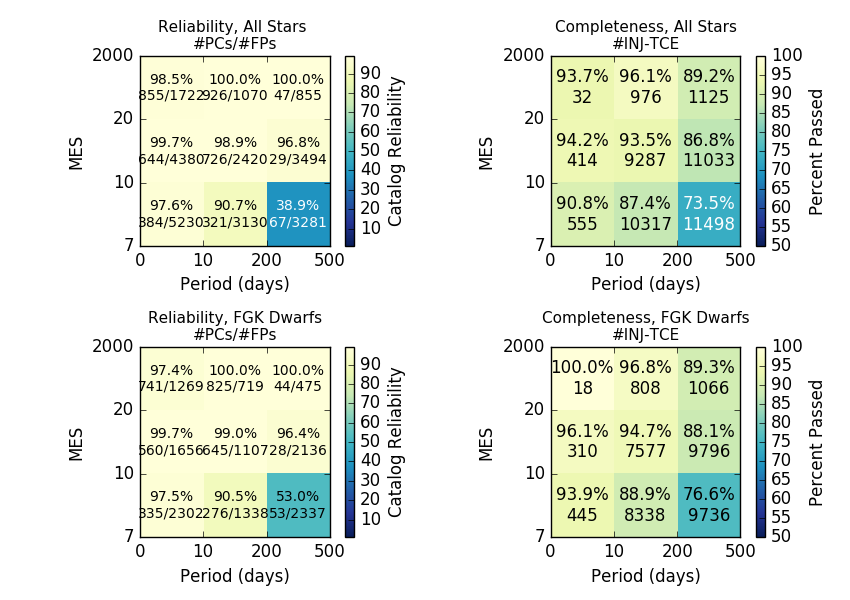
\includegraphics[width=0.95\linewidth]{fig-completeReliabilityCard.png}
\caption{ A coarse binning of the completeness and reliability across period and MES. On the left, the percentage for reliability is given in each box with the number of OPS-PCs and the number of OPS-FPs written below it.  On the right, the percentage for the completeness and the number of \injtce s for that box is given. The bottom two plots give the reliability and completeness just based on the FGK dwarf stars. }
\label{f:scoregrid}
\end{center}
\end{figure*}


%For the later, we use the parameters provided by the supplemental DV fits.  \citet{Christiansen2017} shows that the radii based on the MCMC fits match those of the supplemental DV fits. We do not provided MCMC fits of the entire set of false positives in the \opstce\ set and so cannot use them for our analysis here.

\subsubsection{Completeness}
The completeness of the Robovetter is the fraction of \opstce{s} that are turned into PCs.  We calculate the completeness using the \injtce{s} as explained in \S\ref{injectsec}.  
%We are only measuring the completeness of the Robovetter. If a true transit was not returned by the \Kepler\ pipeline as a TCE, the Robovetter never saw it and it is not part of our completeness measurements. To understand the completeness of the \Kepler\ pipeline see \citet{Christiansen2017} and \citet{Burke2017} [ REFERENCE PAPERS or KSCI's here].  The completeness is calculated using the \ninjtces\ \injtce\ events recovered by the pipeline and discussed in \S\ref{injectsec}.  
Across the entire set of injections, periods ranging from 0.5--500\,d, the completeness is \completeness{} per cent. As expected the completeness of the catalog is higher for transits at shorter periods and higher significance and lower for longer periods and less significant planets. Figure~\ref{f:1dcompare} shows how the completeness varies with Period, MES and number of transits. The small drop in completeness just short of 90\,days is real and is caused by the odd-even metric (\S\ref{s:oddeven})confusing true transits for eclipsing binaries.  

Long period, large radii planets are less complete than the small radii ones, though there is a reduction in completeness as the period increases.  The reason the larger planets appear to be removed at a more efficient rate is because more large planets have long durations and several of our metrics perform less well for long durations. For example, Marshall [something about how the fit works] and the probability of overlapping a cadence impacted by Rolling Band is higher (see Skye). 

[NEED to include the more detailed grid that Jeff has made.]



\subsubsection{Effectiveness}
The effectiveness of the Robovetter at identifying instrumental and stellar noise is calculated as discussed in \S\ref{s:relcalc} using the union of the \invtce s and the \scrtce s. Overall the effectiveness is 99.6 per cent.  Only 119 of the 28,735 simulated false positives are dispositioned by the Robovetter incorrectly (i.e. as a PC).  Unfortunately most of these INV/SCR-PCs fall at long periods and low MES.
%105 have a MES less than 10 and 65 have a period greater than 200\,d. 
Using the 4544 \invtce s and \scrtce s that have periods greater than 200\,d and MES less than 10, the Robovetter's effectiveness is 98.8 per cent.  Unfortunately, because there are so few candidates at these long periods, this translates to a relatively low reliability.

[DO we want a detailed grid of effectiveness in the paper?]

\subsubsection{Reliability}
\label{s:reliability}
The reliability is measured according to the method described in \S\ref{s:relcalc} using the effectiveness number and the number of observed PCs and FPs.  The overall reliability of the catalog is 97 per cent. However, as Figure~\ref{f:1dcompare} demonstrates, the reliability for long period, and especially low MES planets is significantly lower.  For periods longer than 200\,d and MES less than 10, the reliability of the catalog is approximately 39 per cent.

[WE CAN"T do a fine grid for reliability, BUT WE COULD PLot VS THE  OTHER PARAMETERS]

\begin{figure*}[h!]
 \begin{center}
  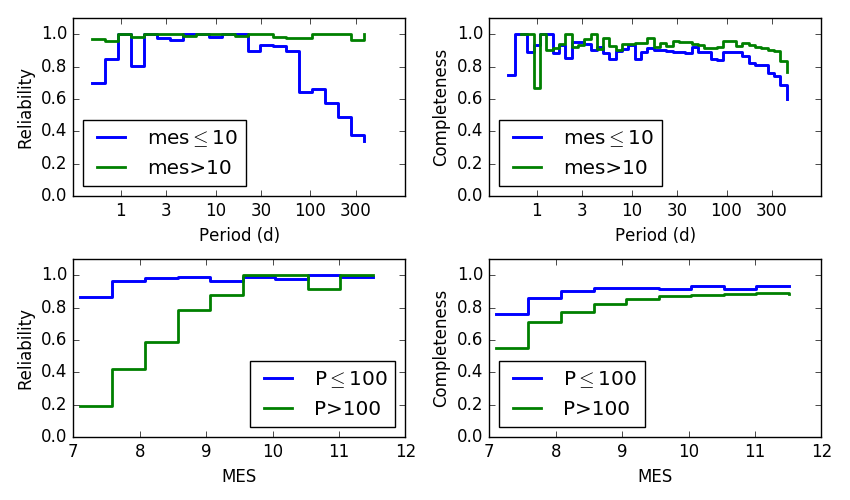
\includegraphics[width=1.0\linewidth]{fig-compRel1D-PerMes.png}
  \caption{ The completeness (right) and reliability (left) of the DR25 catalog plotted for various Period (top) and MES (bottom) bins. [Ntransits was done with NGOOD...I NEED TO CHANGE.] }
  \label{f:1dcompare}
 \end{center}
 \end{figure*}

\begin{figure*}[h!]
\begin{center}
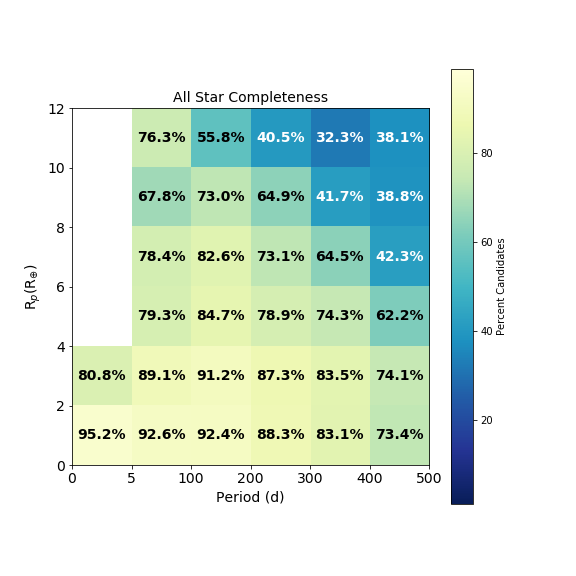
\includegraphics[width=0.45\linewidth]{fig-AllCompletePR.png}
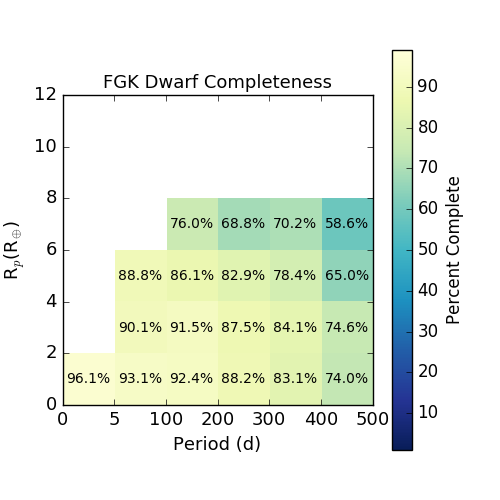
\includegraphics[width=0.45\linewidth]{fig-FgkCompletePR.png}
\caption{A 2D binning of the catalog completeness (this does not include pipeline completeness) of the DR25 candidate catalog for period and planet radius for all stars (left) and for FGK dwarf stars (right). Bins with fewer than 10 recovered \injtce{s} are not plotted.}
\label{f:prCompleteness}
\end{center}
\end{figure*}

\begin{figure*}[h!]
\begin{center}
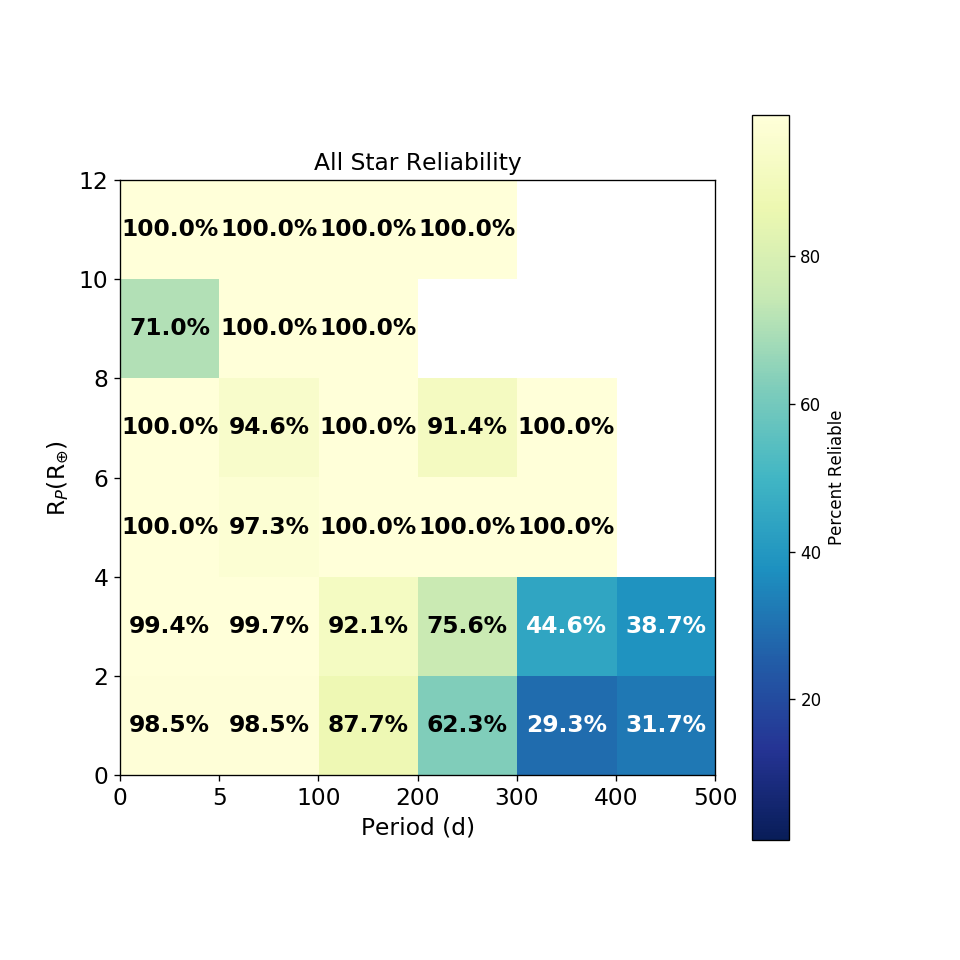
\includegraphics[width=0.45\linewidth]{fig-AllReliabilityPR.png}
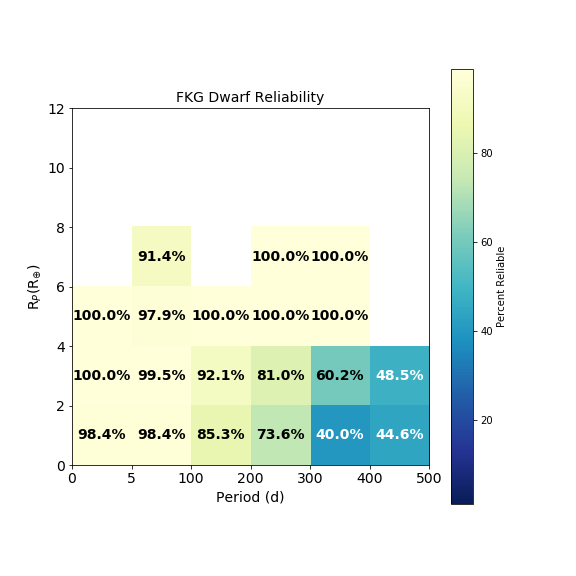
\includegraphics[width=0.45\linewidth]{fig-FgkReliabilityPR.png}
\caption{A 2D binning of the candidate catalog reliability for period and planet radius for all stars (left) and for the FGK dwarf stars (right). Bins with fewer than 3 candidates or fewer than 20 simulated false alarms (from \invtce{} and \scrtce{}) are not plotted.}
\label{f:prReliability}
\end{center}
\end{figure*}



\subsubsection{Adjusted with Disposition Scores}
\label{s:crscores}
The disposition scores discussed in \S\ref{s:scores} can be used to select a more reliable, though more incomplete, sample of planet candidates.  How the completeness and reliability of the catalog vary for different cuts on the disposition score is shown in Figure~\ref{f:adjscore} for MES$<$10 and Period$>$200\,d. 
Notice that the effectiveness of the Robovetter increases as expected as the score threshold is increased.  
The reliability values also depend on the number of OBS-PCs that remain, which is why it does not change in step with the effectiveness.
Selecting PCs by choosing those with a disposition score above 0.6 will yield an 85 per cent reliability with a completeness that is still above 50 per cent. Doing a score cut in this way causes a few \opstce s that are formally called an FP to be promoted to a PC. An FP with a high score occurs when a TCE marginally fails a single metric.

\begin{figure}[h!]
 \begin{center}
  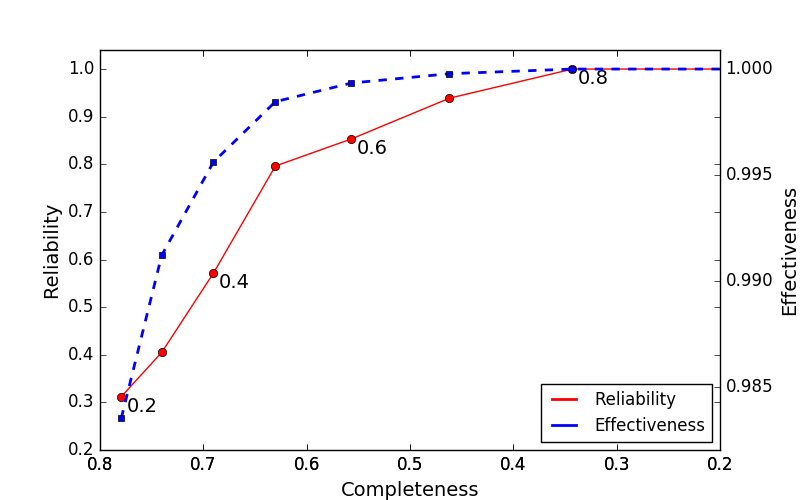
\includegraphics[width=1.0\linewidth]{fig-CRadjustScore-DR25.png}
  \caption{\label{f:adjscore}The reliability (red) and effectiveness (blue) of the MES<10 and periods between 200 and 500\,d planet candidate list that results from determining the candidates by allowing all \opstce s with score values greater than the number shown in black.}
 \end{center}
 \end{figure}


